\documentclass[a4paper]{article}

% Included packages ---------------------------------------------------------- %
\usepackage{inputenc}                 % utf-8 encoding, æ, ø , å, etc.
\usepackage{a4wide}                          % Adjust margins to better fit A4 format.
\usepackage{array}                           % Matrices.
\usepackage{amsmath}                         % Math symbols, and enhanced matrices.
\usepackage{amsfonts}                        % Math fonts.
\usepackage{amssymb}                         % Additional symbols.
\usepackage{wasysym}                         % More additional symbols.
\usepackage{mathrsfs}                        % Most additional symbols.
\usepackage[pdftex]{graphicx}                % Improved inclusion of .pdf-graphics files.
\usepackage{sidecap}                         % Floats with captions to the right/left.
\usepackage{cancel}                          % Visualize cancellations in equations.
\usepackage{enumerate}                       % Change counters (arabic, roman, etc.).
\usepackage{units}                           % Adds better looking fractions (nicefrac).
\usepackage{floatrow}                        % Multi-figure floats.
\usepackage{subfig}                          % Multi-figure floats.
\usepackage{caption}                         % Adds functionality to captions.
\usepackage{bm}                              % Bolded text in math mode.
\usepackage{combinedgraphics}                % Figures; let latex handle the text itself.
\usepackage[framemethod=default]{mdframed}   % Make boxes.
\usepackage{listings}                        % For including source code.
\usepackage[colorlinks]{hyperref}            % Interactive references, colored.
\usepackage{soul}                            % Make vertical bars through text.
\usepackage{nicefrac}                        % Nice fractions with \nicefrac.
\usepackage{mathtools}                       % Underbrackets, overbrackets.
\usepackage{wasysym}                         % \smiley{}-s!
\usepackage{multicol}                        % Multiple text columns.
\usepackage{capt-of}                         % Caption things which are not floats.
\usepackage[url=false]{biblatex}             % Citations (made easy).
\usepackage{simplewick}                      % Contractions using Wick's theorem for QFT.
\usepackage{booktabs}                        % Tables.
\usepackage{bbold}
\usepackage{tikz}

% Differentials -------------------------------------------------------------- %
\newcommand{\dt}{\,\mathrm{d}t}
\newcommand{\dx}{\,\mathrm{d}x}
\newcommand{\dr}{\,\mathrm{d}r}

% Derivatives ---------------------------------------------------------------- %
\newcommand{\der} [2]{\frac{\mathrm{d} #1}{\mathrm{d} #2}}   % Derivative.
\newcommand{\pder}[2]{\frac{\partial #1}{\partial #2}}       % Partial derivative.

% Matrices ------------------------------------------------------------------- %
\newcommand{\mat} [2]{\begin{matrix}[#1] #2 \end{matrix}}    % Nothing enclosing it.
\newcommand{\pmat}[2]{\begin{pmatrix}[#1] #2 \end{pmatrix}}  % Enclosing parentheses.
\newcommand{\bmat}[2]{\begin{bmatrix}[#1] #2 \end{bmatrix}}  % Enclosing square brackets.
\newcommand{\vmat}[2]{\begin{vmatrix}[#1] #2 \end{vmatrix}}  % Enclosing vertical bars.
\newcommand{\Vmat}[2]{\begin{Vmatrix}[#1] #2 \end{Vmatrix}}  % Enclosing double bars.

% Number sets ---------------------------------------------------------------- %
\newcommand{\R}{\mathbb{R}}
\newcommand{\Q}{\mathbb{Q}}
\newcommand{\N}{\mathbb{N}}
\newcommand{\Z}{\mathbb{Z}}
\newcommand{\C}{\mathbb{C}}

% Manually set alignment of rows / columns in matrices (mat, pmat, etc.) ----- %
\makeatletter
\renewcommand*\env@matrix[1][*\c@MaxMatrixCols c]{%
  \hskip -\arraycolsep
  \let\@ifnextchar\new@ifnextchar
  \array{#1}}
\makeatother

% References ----------------------------------------------------------------- %
\newcommand{\Fig}[1]{Fig.\ \ref{fig:#1}}
\newcommand{\fig}[1]{Fig.\ \ref{fig:#1}}
\newcommand{\eq} [1]{Eq.\ (\ref{eq:#1})}
\newcommand{\Eq} [1]{Eq.\ (\ref{eq:#1})}
\newcommand{\tab}[1]{Table \ref{tab:#1}}
\newcommand{\Tab}[1]{Table \ref{tab:#1}}

% Paragraph formatting ------------------------------------------------------- %
\setlength{\parindent}{5.5mm}
\setlength{\parskip}  {0mm}

% Source code listings ------------------------------------------------------- %
\definecolor{commentGreen}{RGB}{34,139,34}
\definecolor{keywordBlue}{RGB}{0,0,255}
\definecolor{stringPurple}{RGB}{160,32,240}
\lstset{language=matlab}
\lstset{basicstyle=\ttfamily\small}
\lstset{frame=single}
\lstset{stringstyle=\color{stringPurple}}
\lstset{keywordstyle=\color{keywordBlue}}
\lstset{commentstyle=\color{commentGreen}}
\lstset{morecomment=[l][\color{commentGreen}\bfseries]{\%\%}}
\lstset{showspaces=false}
\lstset{showstringspaces=false}
\lstset{showtabs=true}
\lstset{columns=fixed}
\lstset{breaklines}
\lstset{literate={~} {$\sim$}{1}}
\lstset{numbers=left}              
\lstset{stepnumber=1}
\renewcommand{\ttdefault}{pcr}
\lstdefinestyle{prt}{frame=none,basicstyle=\ttfamily\small}

% Convenient shorthand notation ---------------------------------------------- %
\newcommand{\nn}{\nonumber}
\newcommand{\e}[1]{\cdot10^{#1}}
\renewcommand{\i}{\hat{\imath}}
\renewcommand{\j}{\hat{\jmath}}
\renewcommand{\k}{\hat{k}}

% Caption position of tables at the top -------------------------------------- %
\floatsetup[table]{capposition=top}

% Black frame with white background ------------------------------------------ %
\newmdenv[linecolor=black,backgroundcolor=white]{exframe}

% Including vector drawings from inkscape ------------------------------------ %
\newenvironment{combFig}[5]{
  \begin{figure}[#1] 
    \centering 
    \includecombinedgraphics[vecscale=#2, keepaspectratio]{#3} 
    \caption{#4 \label{#5}}
  \end{figure}
  }

  {
}

% Including pdf graphics ----------------------------------------------------- %
\newenvironment{pdfFig}[5]{
  \begin{figure}[#1] 
    \centering 
    \includegraphics[width= #2]{#3} 
    \caption{#4 \label{#5}}
  \end{figure}
  }

  {
}

% Exercise and subexercise counters ------------------------------------------ %
\newcounter{excounter}
\renewcommand\theexcounter{\arabic{excounter}}
\newcommand\exlabel{\theexcounter}
\setcounter{excounter}{1}

\newcounter{subexcounter}
\renewcommand\thesubexcounter{\arabic{subexcounter}}
\newcommand\subexlabel{\thesubexcounter}
\setcounter{subexcounter}{1}

% Environments for exercises ------------------------------------------------- %
\newenvironment{exercise}[1]{
  \subsection*{Exercise \theexcounter: #1}
  \setcounter{subexcounter}{1}                      % Reset the subexercise counter to a.
  \addcontentsline{toc}{section}{\theexcounter: #1} % Add the exercise to TOC
  }
      % Exercise text.
  {
  \stepcounter{excounter}                           % Add one to the exercise counter.
  \newpage
}

% Environment for subexercises ----------------------------------------------- %
\newenvironment{subexercise}{
  \begin{exframe}
    \begin{itemize}  \setlength{\itemindent}{1cm}
      \item[{\bf Exercise \thesubexcounter}] 
	}
	  % Subexercise text.
	{
    \end{itemize}
  \end{exframe}
  \stepcounter{subexcounter}                        % Add one to the exercise counter.
}

% Environment for proofs ----------------------------------------------------- %
\newenvironment{proof}[2]{
  \begin{exframe}
    \begin{itemize}  \setlength{\itemindent}{0.6cm}
      \item[{\bf #1} {\bf #2}] 
	}
	  % Subexercise text.
	{
    \end{itemize}
  \end{exframe}
}

% Environment for answers ---------------------------------------------------- %
\newenvironment{answer}{}{}

% Set bibliography file and path for images.
\bibliography{references/fys4180ref.bib}
\graphicspath{{./images/}}
\newcommand{\includepdfgraphics}[2]{\includecombinedgraphics[#1]{./images/#2}}



\renewcommand{\L}{\hat{L}_z}
\renewcommand{\S}{\hat{S}_z}
\newcommand{\slater}{|P_1P_2\dots P_N\rangle}
\newcommand{\cm}{c_\mu}
\newcommand{\cn}{c_\nu}
\newcommand{\cmd}{c_\mu^\dagger}
\newcommand{\cnd}{c_\nu^\dagger}
\newcommand{\ca}{c_\alpha}
\newcommand{\cad}{c_\alpha^\dagger}
\newcommand{\cb}{c_\beta}
\newcommand{\cbd}{c_\beta^\dagger}

\renewcommand{\u}[1]{{\bf #1}_\uparrow}
\renewcommand{\d}[1]{{\bf #1}_\downarrow}

\newcommand{\boud}{b_{\u{1}}^\dagger}
\newcommand{\bou}{b_{\u{1}}}
\newcommand{\bodd}{b_{\d{1}}^\dagger}
\newcommand{\bod}{b_{\d{1}}}

\newcommand{\bfud}{b_{\u{5}}^\dagger}
\newcommand{\bfu}{b_{\u{5}}}
\newcommand{\bfdd}{b_{\d{5}}^\dagger}
\newcommand{\bfd}{b_{\d{5}}}


% Title
\title{FYS-KJM4480 Project 1}
\date{}
\author{Morten Ledum}
% ---------------------------------------------------------------------------- %
% ---------------------------------------------------------------------------- %
\begin{document}
\maketitle
\subsection*{Exercise 1}
\begin{exframe}
\begin{itemize}
  \item[1a)] Let $c_p^\dagger$ and $c_p$ be creation and annihilation operators for the spin-orbitals $\phi_p$. 

  Define the second quantized form of the operators $\hat{L}_z$ and $\hat{S}_z$. Use that the spin-orbitals are eigenfunctions to simplify.
\end{itemize}
\end{exframe}
Both $\hat{L}_z$ and $\hat{S}_z$ are one-body operators. Since we know that a general operator, $\hat{A}$, takes the form 
\begin{align}
\hat{A}=\sum_{\mu \nu} \langle \mu | \hat a | \nu \rangle c^\dagger_\mu c_\nu,
\end{align}
after second quantization, we may simply apply this to $\hat{L}_z$ and $\hat{S}_z$. Doing this yields, for $\hat{L}_z$, 
\begin{align}
\hat{L}_z &= \sum_{\mu \nu} \langle \mu | \hat{l}_z | \nu \rangle c^\dagger_\mu c_\nu =  \sum_{\mu \nu} \langle \mu | \hbar m_\nu | \nu \rangle c^\dagger_\mu c_\nu \nn\\
&= \sum_{\mu \nu} \hbar m_\nu \underbrace{\langle \mu |  \nu \rangle}_{\delta_{\mu \nu}} c^\dagger_\mu c_\nu = \sum_{\mu} \hbar m_\mu c^\dagger_\mu c_\mu.
\end{align}
An analogous treatment of $\hat{S}_z$ gives 
\begin{align}
\hat{S}_z &= \sum_{\mu} \hbar \alpha_\mu c^\dagger_\mu c_\mu. 
\end{align}


\begin{exframe}
\begin{itemize}
  \item[1b)] Show that any Slater determinant, $|P_1P_2\dots P_N\rangle$ is an eignefunction for $\L$ with eigenvalue $\hbar M=\hbar\sum_i m_i$, where $m_i=m_{p_i}$. Show that the Slater determinant is also an eigenfunction for $\S$ with eigenvalue $\hbar S_z=\hbar\sum_i\alpha_i$, with $\alpha_i=\alpha_{p_i}$.
\end{itemize}
\end{exframe}
Using the expressions from exercise 1a), and letting the index $i=1,2,\dots,N$ denote the occupied spin-orbitals in the Slater determinant, we find for $\L$
\begin{align}
\L \slater  &= \sum_{\mu} \hbar m_\mu c^\dagger_\mu c_\mu \slater \nn\\
            &= \sum_{i=1}^N \hbar  m_i c^\dagger_i c_i \slater \nn\\
            &= \hbar \sum_{i=1}^N m_i \slater = \hbar M \slater,
\end{align}
where we have used that acting on the Slater determinant with $c_\mu$ yields zero for any $\mu\not=P_i$ for any $i$ (i.e. any not-occupied spin-orbital $\mu$). The same argument may be applied to $\S$, which gives
\begin{align}
\S \slater &= \hbar \sum_{i=1}^N \alpha_i \slater = \hbar S_z \slater.
\end{align}
This shows that the Slater determinant, $\slater$, is a simultaneous eigenfunction for both $\L$ and $\S$.

\begin{exframe}
\begin{itemize}
  \item[1c)] Show that 
  \begin{align}
  \left[\S,\L \right] = 0.
  \end{align}
\end{itemize}
\end{exframe}
We may do this by considering the form of $\L$ and $\S$ found in exercise 1a), and the fundamental anti-commutator relations\footnote{This can also be done by considering the action of $[\S,\L]$ on a Slater determinant, $\slater$, but that is a lot less fun!}
\begin{align}
\left\{c_\mu, c_\nu^\dagger\right\} = \delta_{\mu \nu}, \ \ \ \text{ and } \ \ \ \left\{c_\mu^\dagger, c_\nu^\dagger\right\} = \left\{c_\mu, c_\nu\right\} = 0. \label{eq:1}
\end{align}
We expand the commutator, $[\S,\L]=\S\L-\L\S$, and consider the first term. We will show that this term equals the second term. Doing this, we find
\begin{align}
\S\L  &= \left(\sum_{\mu}\hbar\alpha_\mu c_\mu^\dagger c_\mu \right)\left(\sum_{\nu}\hbar m_\nu c_\nu^\dagger c_\nu \right) \nn\\
      &= \hbar^2 \sum_\mu \sum_\nu \alpha_\mu m_\nu   c_\mu^\dagger c_\mu c_\nu^\dagger c_\nu. \label{eq:2}
\end{align}
Let us now commute the creation and annihilation operators past each other according to \eq{1},
\begin{align}
c_\mu^\dagger c_\mu c_\nu^\dagger c_\nu &= \cmd (-\cnd\cm+\delta_{\mu\nu}) \cn \nn\\
                                        &= - \cmd \cnd \cm \cn + \cmd \cn \delta_{\mu\nu} \nn\\
                                        &= - (-\cnd\cmd) \cm \cn + \cmd \cn \delta_{\mu\nu} \nn\\
                                        &= \cnd\cmd (-\cn\cm) + \cmd \cn \delta_{\mu\nu} \nn\\
                                        &= -\cnd(-\cn\cmd+\delta_{\mu\nu})\cm + \cmd \cn \delta_{\mu\nu} \nn\\
                                        &= \cnd\cn\cmd\cm - \cancel{\cnd\cm\delta_{\mu\nu}} + \cancel{\cmd \cn \delta_{\mu\nu}} \nn\\
                                        &= \cnd\cn\cmd\cm.
\end{align}
Inserting this back into \eq{2} we find that 
\begin{align}
\S\L  &= \hbar^2 \sum_\mu \sum_\nu \alpha_\mu m_\nu   c_\mu^\dagger c_\mu c_\nu^\dagger c_\nu \nn\\
      &= \hbar^2 \sum_\mu \sum_\nu \alpha_\mu m_\nu  \cnd\cn\cmd\cm  \nn\\
      &= \left(\sum_\nu \hbar m_\nu \cnd\cn \right) \left(\sum_\mu \hbar\alpha_\mu \cmd\cm \right)= \L\S,
\end{align}
which proves that $[\S\L]=0$. We note that this all depends on the orthonormality of the spin-orbital basis chosen.


\newpage
\subsection*{Exercise 2}
We can transform the Hamiltonian to dimensionless form by introducing a suitable set of units. We will compute in a set of units where
\begin{align}
\hbar=m_e=ke^2=\omega=1.
\end{align}
\begin{exframe}
\begin{itemize}
  \item[2a)] We start with the two-electron system and define our single particle Hilbert space to consist of the orbitals $(n=0,m=0)$, $(n=1,n=0)$, $(n=0, m=\pm1)$, and $(n=0, m=\pm2)$, with their corresponding spin degeneracies. Without spin we have thus six single-particle states. Adding the two spin degeneracies, we end up with $12$ states.

  Set up the $M=S_z=0$ ground state of the non-interacting problem ($\hat{H}_0$) as a reference Slater determinant $|\Phi\rangle$. Use second quantization. Define the fermi level/energy. Draw a diagram of the reference state.
\end{itemize}
\end{exframe}
\begin{SCfigure}
\begin{tikzpicture}[scale=0.6]
  \draw[->] (-3.5,-1) -- (3.5,-1) node[anchor=west] {$m$};
  \draw[->] (-3.5,-1) -- (-3.5,3) node[anchor=south] {$e$};
  \draw (-3.6,0) node[anchor=east] {$1\omega$} -- (-3.4,0);
  \draw (-3.6,1) node[anchor=east] {$2\omega$} -- (-3.4,1);
  \draw (-3.6,2) node[anchor=east] {$3\omega$} -- (-3.4,2);
  \draw (-2,-1.2) node[anchor=north] {$-2$} -- (-2,-.8);
  \draw (-1,-1.2) node[anchor=north] {$-1$} -- (-1,-.8);
  \draw (0,-1.2) node[anchor=north] {$0$} -- (0,-.8);
  \draw (0,-1.2) node[anchor=north] {$0$} -- (0,-.8);
  \draw (1,-1.2) node[anchor=north] {$+1$} -- (1,-.8);
  \draw (2,-1.2) node[anchor=north] {$+2$} -- (2,-.8);
  \begin{scope}
    \draw (-.5,0) -- (.5,0);
    \draw[->] (-.25,-.25) node[anchor=north]{$1$} -- (-.25,.25);
    \draw[<-] (.25,-.25) node[anchor=north]{$2$} -- (.25,.25);
  \end{scope}
  \begin{scope}[xshift=-1cm,yshift=1cm]
    \draw (-.5,0) -- (.5,0);
  \end{scope}
  \begin{scope}[xshift=1cm,yshift=1cm]
    \draw (-.5,0) -- (.5,0);
  \end{scope}
  \begin{scope}[xshift=-2cm,yshift=2cm]
    \draw (-.5,0) -- (.5,0);
  \end{scope}
  \begin{scope}[xshift=0cm,yshift=2cm]
    \draw (-.5,0) -- (.5,0);
  \end{scope}
  \begin{scope}[xshift=2cm,yshift=2cm]
    \draw (-.5,0) -- (.5,0);
  \end{scope}
\end{tikzpicture}
\caption{Ground state of the non-interacting problem, the reference Slater determinant $|\Phi\rangle$. The two electrons occupy the $\u{1}$ and $\d{1}$ spin-orbitals.}
\label{fig:gs}
\end{SCfigure}
Using the new set of units, the Hamiltonian takes the form 
\begin{align}
\hat{H} = \hat{H}_0 + \hat{W} = \sum_{i=1}^n \left( \frac{-\nabla^2}{2} +\frac{1}{2}r_i^2\right) + \sum_{i=1}^n\sum_{j=i+1}^n\frac{1}{|{\bf r}_i-{\bf r}_j|}.
\end{align}
Second quantization of this Hamiltonian yields
\begin{align}
\hat{H} = \underbrace{\sum_\mu\sum_\nu \langle \mu | \hat{h} | \nu \rangle \cmd \cn}_{\hat{H}_0} + \underbrace{\frac{1}{4}\sum_\mu\sum_\nu\sum_\alpha\sum_\beta \langle \mu\nu|\hat{w}| \alpha \beta \rangle \cmd\cnd \cb\ca}_{\hat{W}}, \label{eq:3}
\end{align}
where we have used the general form of a two-body operator, $\hat{A}$ under second quantization, $\hat{A}=\sum_{\mu\nu\alpha\beta} \langle \mu\nu|\hat{a}|\alpha\beta\rangle \cmd\cnd\cb\ca$. For the two-electron non-interacting problem, we may find the ground state Slater determinant by considering the action of $\hat{H}_0$ on $\slater$:
\begin{align}
\hat{H}_0 \slater &= \sum_\mu\sum_\nu \langle \mu | \hat{h} | \nu \rangle \cmd \cn \slater \nn\\
                  &= \sum_\mu\sum_i \langle \mu | \varepsilon_i | i \rangle \cmd c_i \slater \nn\\
                  &= \sum_\mu\sum_i \varepsilon_i \underbrace{\langle \mu | i \rangle}_{\delta_{\mu i}} \cmd c_i \slater \nn\\
                  &= \sum_i \varepsilon_i c_i^\dagger c_i \slater,
\end{align}
where we once again have used the fact that operating on $\slater$ with any $c_\mu$ with $\mu\not=P_i$ yields zero. Hence the index $i$ denotes only the occupied spin-orbitals in the Slater determinant. Please note that $\varepsilon_i$ is shorthand notation for $\varepsilon_{n_i m_i}$. 


\newcommand{\ra}[1]{\renewcommand{\arraystretch}{#1}}
\begin{table*}\centering
%\ra{1.0}
\begin{tabular}{@{}llllllllll@{}}\toprule
Spin-         & Spin-orbital        & spatial         & Radial quantum    & Azimutal quantum    & Spin                       \\
orbital       & index               & index, $p(n,m)$ & number, $n$       & number, $m$         & projection, $\alpha$       \\
\midrule
$\u{1}$       & 1                   & 1               & 0                 & $\phantom{-}0$      & $\phantom{-}\hbar/2$                        \\
$\d{1}$       & 2                   & 1               & 0                 & $\phantom{-}0$      & $-\hbar/2$                        \\
$\u{2}$       & 3                   & 2               & 0                 & $-1$                & $\phantom{-}\hbar/2$                        \\
$\d{2}$       & 4                   & 2               & 0                 & $-1$                & $-\hbar/2$                        \\
$\u{3}$       & 5                   & 3               & 0                 & $+1$                & $\phantom{-}\hbar/2$                        \\
$\d{3}$       & 6                   & 3               & 0                 & $+1$                & $-\hbar/2$                        \\
$\u{4}$       & 7                   & 4               & 0                 & $-2$                & $\phantom{-}\hbar/2$                        \\
$\d{4}$       & 8                   & 4               & 0                 & $-2$                & $-\hbar/2$                        \\
$\u{5}$       & 9                   & 5               & 1                 & $\phantom{-}0$      & $\phantom{-}\hbar/2$                        \\
$\d{5}$       & 10                  & 5               & 1                 & $\phantom{-}0$      & $-\hbar/2$                        \\
$\u{6}$       & 11                  & 6               & 0                 & $+2$                & $\phantom{-}\hbar/2$                        \\
$\d{6}$       & 12                  & 6               & 0                 & $+2$                & $-\hbar/2$                        \\
\bottomrule
\end{tabular}
\caption{Notation used to denote the spin-orbitals used throughout the project report.\label{tab:1}}
\end{table*}

We know the form of the single-particle energies, $\varepsilon_{n m}=(2n+|m|+1)/2$, and thus it is easy to see that the lowest energy state for the non-interacting two-electron problem is obtained by placing both electrons in the $n=m=0$ orbital. In the rest of the project we will use the notation found in \tab{1} to denote the spin-orbitals. Using this notation, we are placing the elctrons in the spin-orbitals $\u{1}$ and $\d{1}$, i.e. $|\Phi\rangle = |\u{1}\d{1}\rangle$. This state has energy $E_0^{(2)}=2$, since $\hat{H}_0|\u{1}\d{1}\rangle=2|\u{1}\d{1}\rangle$. The state is shown in \fig{gs} in so called Fock-Darwin representation.

The fermi level is defined as the single particle energy of the highest energy occupied spin-orbital in the Slater determinant. In our case, $E^{(2)}_f=1$. We note that any spin-orbital with energy at or below the fermi level is occupied, while corresponding spin-orbitals with energies above the fermi level are unoccupied.

\begin{exframe}
\begin{itemize}
  \item[\phantom{2a)}] Define quasiparticle creation-, and annihilation operators for this problem. Construct thereafter er all possible one-particle-one-hole excitations $|\Phi^A_I\rangle$, where $I$ is an index below the fermi level, and $A$ is an index above it. Write the Slater determinants in terms of quasiparticle creation-, and annihilation operators. Ensure that you only write down the states that have $M=S_z=0$. Draw diagrams.

  Construct thereafter all possible two-particle-two-hole excitations $|\Phi_{IJ}^{AB}\rangle$ in a similar manner. Draw diagrams and make sure to again only include states with $M=S_z=0$. 
\end{itemize}
\end{exframe}
\begin{figure}[p]
\begin{center}
\begin{tikzpicture}[scale=0.6]
  \draw[->] (-3.5,-1) -- (3.5,-1) node[anchor=west] {$m$};
  \draw[->] (-3.5,-1) -- (-3.5,3) node[anchor=south] {$e$};
  \draw (-3.6,0) node[anchor=east] {$1\omega$} -- (-3.4,0);
  \draw (-3.6,1) node[anchor=east] {$2\omega$} -- (-3.4,1);
  \draw (-3.6,2) node[anchor=east] {$3\omega$} -- (-3.4,2);
  \draw (-2,-1.2) node[anchor=north] {$-2$} -- (-2,-.8);
  \draw (-1,-1.2) node[anchor=north] {$-1$} -- (-1,-.8);
  \draw (0,-1.2) node[anchor=north] {$0$} -- (0,-.8);
  \draw (0,-1.2) node[anchor=north] {$0$} -- (0,-.8);
  \draw (1,-1.2) node[anchor=north] {$+1$} -- (1,-.8);
  \draw (2,-1.2) node[anchor=north] {$+2$} -- (2,-.8);
  \begin{scope}
    \draw (-.5,0) -- (.5,0);
    \draw[->] (-.25,-.25) node[anchor=north]{$1$} -- (-.25,.25);
  \end{scope}
  \begin{scope}[xshift=-1cm,yshift=1cm]
    \draw (-.5,0) -- (.5,0);
  \end{scope}
  \begin{scope}[xshift=1cm,yshift=1cm]
    \draw (-.5,0) -- (.5,0);
  \end{scope}
  \begin{scope}[xshift=-2cm,yshift=2cm]
    \draw (-.5,0) -- (.5,0);
  \end{scope}
  \begin{scope}[xshift=0cm,yshift=2cm]
    \draw (-.5,0) -- (.5,0);
    \draw[<-] (.25,-.25) node[anchor=north]{$10$} -- (.25,.25);
  \end{scope}
  \begin{scope}[xshift=2cm,yshift=2cm]
    \draw (-.5,0) -- (.5,0);
  \end{scope}
\end{tikzpicture}
\begin{tikzpicture}[scale=0.6]
  \draw[->] (-3.5,-1) -- (3.5,-1) node[anchor=west] {$m$};
  \draw[->] (-3.5,-1) -- (-3.5,3) node[anchor=south] {$e$};
  \draw (-3.6,0) node[anchor=east] {$1\omega$} -- (-3.4,0);
  \draw (-3.6,1) node[anchor=east] {$2\omega$} -- (-3.4,1);
  \draw (-3.6,2) node[anchor=east] {$3\omega$} -- (-3.4,2);
  \draw (-2,-1.2) node[anchor=north] {$-2$} -- (-2,-.8);
  \draw (-1,-1.2) node[anchor=north] {$-1$} -- (-1,-.8);
  \draw (0,-1.2) node[anchor=north] {$0$} -- (0,-.8);
  \draw (0,-1.2) node[anchor=north] {$0$} -- (0,-.8);
  \draw (1,-1.2) node[anchor=north] {$+1$} -- (1,-.8);
  \draw (2,-1.2) node[anchor=north] {$+2$} -- (2,-.8);
  \begin{scope}
    \draw (-.5,0) -- (.5,0);
    \draw[<-] (.25,-.25) node[anchor=north]{$2$} -- (.25,.25);
  \end{scope}
  \begin{scope}[xshift=-1cm,yshift=1cm]
    \draw (-.5,0) -- (.5,0);
  \end{scope}
  \begin{scope}[xshift=1cm,yshift=1cm]
    \draw (-.5,0) -- (.5,0);
  \end{scope}
  \begin{scope}[xshift=-2cm,yshift=2cm]
    \draw (-.5,0) -- (.5,0);
  \end{scope}
  \begin{scope}[xshift=0cm,yshift=2cm]
    \draw (-.5,0) -- (.5,0);
    \draw[->] (-.25,-.25) node[anchor=north]{$9$} -- (-.25,.25);
  \end{scope}
  \begin{scope}[xshift=2cm,yshift=2cm]
    \draw (-.5,0) -- (.5,0);
  \end{scope}
\end{tikzpicture}
\caption{The two allowed one-particle-one-hole excitations of the $S_z=M=0$ two-electron system, $|\Phi^{\d{5}}_{\d{1}}\rangle$ (left) and $|\Phi_{\u{1}}^{\u{5}}\rangle$ (right). }
\label{fig:2}
\end{center}
\end{figure}
\begin{figure}[p]
\begin{center}
\begin{tikzpicture}[scale=0.6]
  \draw[->] (-3.5,-1) -- (3.5,-1) node[anchor=west] {$m$};
  \draw[->] (-3.5,-1) -- (-3.5,3) node[anchor=south] {$e$};
  \draw (-3.6,0) node[anchor=east] {$1\omega$} -- (-3.4,0);
  \draw (-3.6,1) node[anchor=east] {$2\omega$} -- (-3.4,1);
  \draw (-3.6,2) node[anchor=east] {$3\omega$} -- (-3.4,2);

  \draw (-2,-1.2) node[anchor=north] {$-2$} -- (-2,-.8);
  \draw (-1,-1.2) node[anchor=north] {$-1$} -- (-1,-.8);
  \draw (0,-1.2) node[anchor=north] {$0$} -- (0,-.8);
  \draw (0,-1.2) node[anchor=north] {$0$} -- (0,-.8);
  \draw (1,-1.2) node[anchor=north] {$+1$} -- (1,-.8);
  \draw (2,-1.2) node[anchor=north] {$+2$} -- (2,-.8);

  \begin{scope}
    \draw (-.5,0) -- (.5,0);
    %\draw[->] (-.25,-.25) node[anchor=north]{$1$} -- (-.25,.25);
    %\draw[<-] (.25,-.25) node[anchor=north]{$2$} -- (.25,.25);
  \end{scope}

  \begin{scope}[xshift=-1cm,yshift=1cm]
    \draw (-.5,0) -- (.5,0);
    %\draw[->] (-.25,-.25) node[anchor=north]{$3$} -- (-.25,.25);
    %\draw[<-] (.25,-.25) node[anchor=north]{$4$} -- (.25,.25);
  \end{scope}


  \begin{scope}[xshift=1cm,yshift=1cm]
    \draw (-.5,0) -- (.5,0);
    %\draw[->] (-.25,-.25) node[anchor=north]{$5$} -- (-.25,.25);
    %\draw[<-] (.25,-.25) node[anchor=north]{$6$} -- (.25,.25);
  \end{scope}


  \begin{scope}[xshift=-2cm,yshift=2cm]
    \draw (-.5,0) -- (.5,0);
    %\draw[->] (-.25,-.25) node[anchor=north]{$7$} -- (-.25,.25);
    %\draw[<-] (.25,-.25) node[anchor=north]{$8$} -- (.25,.25);
  \end{scope}


  \begin{scope}[xshift=0cm,yshift=2cm]
    \draw (-.5,0) -- (.5,0);
    \draw[->] (-.25,-.25) node[anchor=north]{$9$} -- (-.25,.25);
    \draw[<-] (.25,-.25) node[anchor=north]{$10$} -- (.25,.25);
  \end{scope}


  \begin{scope}[xshift=2cm,yshift=2cm]
    \draw (-.5,0) -- (.5,0);
    %\draw[->] (-.25,-.25) node[anchor=north]{$11$} -- (-.25,.25);
    %\draw[<-] (.25,-.25) node[anchor=north]{$12$} -- (.25,.25);
  \end{scope}
\end{tikzpicture}
\begin{tikzpicture}[scale=0.6]
  \draw[->] (-3.5,-1) -- (3.5,-1) node[anchor=west] {$m$};
  \draw[->] (-3.5,-1) -- (-3.5,3) node[anchor=south] {$e$};

  \draw (-3.6,0) node[anchor=east] {$1\omega$} -- (-3.4,0);
  \draw (-3.6,1) node[anchor=east] {$2\omega$} -- (-3.4,1);
  \draw (-3.6,2) node[anchor=east] {$3\omega$} -- (-3.4,2);

  \draw (-2,-1.2) node[anchor=north] {$-2$} -- (-2,-.8);
  \draw (-1,-1.2) node[anchor=north] {$-1$} -- (-1,-.8);
  \draw (0,-1.2) node[anchor=north] {$0$} -- (0,-.8);
  \draw (0,-1.2) node[anchor=north] {$0$} -- (0,-.8);
  \draw (1,-1.2) node[anchor=north] {$+1$} -- (1,-.8);
  \draw (2,-1.2) node[anchor=north] {$+2$} -- (2,-.8);

  \begin{scope}
    \draw (-.5,0) -- (.5,0);
    %\draw[->] (-.25,-.25) node[anchor=north]{$1$} -- (-.25,.25);
    %\draw[<-] (.25,-.25) node[anchor=north]{$2$} -- (.25,.25);
  \end{scope}

  \begin{scope}[xshift=-1cm,yshift=1cm]
    \draw (-.5,0) -- (.5,0);
    %\draw[->] (-.25,-.25) node[anchor=north]{$3$} -- (-.25,.25);
    %\draw[<-] (.25,-.25) node[anchor=north]{$4$} -- (.25,.25);
  \end{scope}


  \begin{scope}[xshift=1cm,yshift=1cm]
    \draw (-.5,0) -- (.5,0);
    %\draw[->] (-.25,-.25) node[anchor=north]{$5$} -- (-.25,.25);
    %\draw[<-] (.25,-.25) node[anchor=north]{$6$} -- (.25,.25);
  \end{scope}


  \begin{scope}[xshift=-2cm,yshift=2cm]
    \draw (-.5,0) -- (.5,0);
    \draw[->] (-.25,-.25) node[anchor=north]{$7$} -- (-.25,.25);
    %\draw[<-] (.25,-.25) node[anchor=north]{$8$} -- (.25,.25);
  \end{scope}


  \begin{scope}[xshift=0cm,yshift=2cm]
    \draw (-.5,0) -- (.5,0);
    %\draw[->] (-.25,-.25) node[anchor=north]{$9$} -- (-.25,.25);
    %\draw[<-] (.25,-.25) node[anchor=north]{$10$} -- (.25,.25);
  \end{scope}


  \begin{scope}[xshift=2cm,yshift=2cm]
    \draw (-.5,0) -- (.5,0);
    %\draw[->] (-.25,-.25) node[anchor=north]{$11$} -- (-.25,.25);
    \draw[<-] (.25,-.25) node[anchor=north]{$12$} -- (.25,.25);
  \end{scope}

\end{tikzpicture}
\begin{tikzpicture}[scale=0.6]
  \draw[->] (-3.5,-1) -- (3.5,-1) node[anchor=west] {$m$};
  \draw[->] (-3.5,-1) -- (-3.5,3) node[anchor=south] {$e$};

  \draw (-3.6,0) node[anchor=east] {$1\omega$} -- (-3.4,0);
  \draw (-3.6,1) node[anchor=east] {$2\omega$} -- (-3.4,1);
  \draw (-3.6,2) node[anchor=east] {$3\omega$} -- (-3.4,2);

  \draw (-2,-1.2) node[anchor=north] {$-2$} -- (-2,-.8);
  \draw (-1,-1.2) node[anchor=north] {$-1$} -- (-1,-.8);
  \draw (0,-1.2) node[anchor=north] {$0$} -- (0,-.8);
  \draw (0,-1.2) node[anchor=north] {$0$} -- (0,-.8);
  \draw (1,-1.2) node[anchor=north] {$+1$} -- (1,-.8);
  \draw (2,-1.2) node[anchor=north] {$+2$} -- (2,-.8);

  \begin{scope}
    \draw (-.5,0) -- (.5,0);
    %\draw[->] (-.25,-.25) node[anchor=north]{$1$} -- (-.25,.25);
    %\draw[<-] (.25,-.25) node[anchor=north]{$2$} -- (.25,.25);
  \end{scope}

  \begin{scope}[xshift=-1cm,yshift=1cm]
    \draw (-.5,0) -- (.5,0);
    %\draw[->] (-.25,-.25) node[anchor=north]{$3$} -- (-.25,.25);
    %\draw[<-] (.25,-.25) node[anchor=north]{$4$} -- (.25,.25);
  \end{scope}


  \begin{scope}[xshift=1cm,yshift=1cm]
    \draw (-.5,0) -- (.5,0);
    %\draw[->] (-.25,-.25) node[anchor=north]{$5$} -- (-.25,.25);
    %\draw[<-] (.25,-.25) node[anchor=north]{$6$} -- (.25,.25);
  \end{scope}


  \begin{scope}[xshift=-2cm,yshift=2cm]
    \draw (-.5,0) -- (.5,0);
    %\draw[->] (-.25,-.25) node[anchor=north]{$7$} -- (-.25,.25);
    \draw[<-] (.25,-.25) node[anchor=north]{$8$} -- (.25,.25);
  \end{scope}


  \begin{scope}[xshift=0cm,yshift=2cm]
    \draw (-.5,0) -- (.5,0);
    %\draw[->] (-.25,-.25) node[anchor=north]{$9$} -- (-.25,.25);
    %\draw[<-] (.25,-.25) node[anchor=north]{$10$} -- (.25,.25);
  \end{scope}


  \begin{scope}[xshift=2cm,yshift=2cm]
    \draw (-.5,0) -- (.5,0);
    \draw[->] (-.25,-.25) node[anchor=north]{$11$} -- (-.25,.25);
    %\draw[<-] (.25,-.25) node[anchor=north]{$12$} -- (.25,.25);
  \end{scope}
  \end{tikzpicture}
  \begin{tikzpicture}[scale=0.6]
  \draw[->] (-3.5,-1) -- (3.5,-1) node[anchor=west] {$m$};
  \draw[->] (-3.5,-1) -- (-3.5,3) node[anchor=south] {$e$};

  \draw (-3.6,0) node[anchor=east] {$1\omega$} -- (-3.4,0);
  \draw (-3.6,1) node[anchor=east] {$2\omega$} -- (-3.4,1);
  \draw (-3.6,2) node[anchor=east] {$3\omega$} -- (-3.4,2);

  \draw (-2,-1.2) node[anchor=north] {$-2$} -- (-2,-.8);
  \draw (-1,-1.2) node[anchor=north] {$-1$} -- (-1,-.8);
  \draw (0,-1.2) node[anchor=north] {$0$} -- (0,-.8);
  \draw (0,-1.2) node[anchor=north] {$0$} -- (0,-.8);
  \draw (1,-1.2) node[anchor=north] {$+1$} -- (1,-.8);
  \draw (2,-1.2) node[anchor=north] {$+2$} -- (2,-.8);

  \begin{scope}
    \draw (-.5,0) -- (.5,0);
    %\draw[->] (-.25,-.25) node[anchor=north]{$1$} -- (-.25,.25);
    %\draw[<-] (.25,-.25) node[anchor=north]{$2$} -- (.25,.25);
  \end{scope}

  \begin{scope}[xshift=-1cm,yshift=1cm]
    \draw (-.5,0) -- (.5,0);
    \draw[->] (-.25,-.25) node[anchor=north]{$3$} -- (-.25,.25);
    %\draw[<-] (.25,-.25) node[anchor=north]{$4$} -- (.25,.25);
  \end{scope}


  \begin{scope}[xshift=1cm,yshift=1cm]
    \draw (-.5,0) -- (.5,0);
    %\draw[->] (-.25,-.25) node[anchor=north]{$5$} -- (-.25,.25);
    \draw[<-] (.25,-.25) node[anchor=north]{$6$} -- (.25,.25);
  \end{scope}


  \begin{scope}[xshift=-2cm,yshift=2cm]
    \draw (-.5,0) -- (.5,0);
    %\draw[->] (-.25,-.25) node[anchor=north]{$7$} -- (-.25,.25);
    %\draw[<-] (.25,-.25) node[anchor=north]{$8$} -- (.25,.25);
  \end{scope}


  \begin{scope}[xshift=0cm,yshift=2cm]
    \draw (-.5,0) -- (.5,0);
    %\draw[->] (-.25,-.25) node[anchor=north]{$9$} -- (-.25,.25);
    %\draw[<-] (.25,-.25) node[anchor=north]{$10$} -- (.25,.25);
  \end{scope}


  \begin{scope}[xshift=2cm,yshift=2cm]
    \draw (-.5,0) -- (.5,0);
    %\draw[->] (-.25,-.25) node[anchor=north]{$11$} -- (-.25,.25);
    %\draw[<-] (.25,-.25) node[anchor=north]{$12$} -- (.25,.25);
  \end{scope}
\end{tikzpicture}
  \begin{tikzpicture}[scale=0.6]
  \draw[->] (-3.5,-1) -- (3.5,-1) node[anchor=west] {$m$};
  \draw[->] (-3.5,-1) -- (-3.5,3) node[anchor=south] {$e$};

  \draw (-3.6,0) node[anchor=east] {$1\omega$} -- (-3.4,0);
  \draw (-3.6,1) node[anchor=east] {$2\omega$} -- (-3.4,1);
  \draw (-3.6,2) node[anchor=east] {$3\omega$} -- (-3.4,2);

  \draw (-2,-1.2) node[anchor=north] {$-2$} -- (-2,-.8);
  \draw (-1,-1.2) node[anchor=north] {$-1$} -- (-1,-.8);
  \draw (0,-1.2) node[anchor=north] {$0$} -- (0,-.8);
  \draw (0,-1.2) node[anchor=north] {$0$} -- (0,-.8);
  \draw (1,-1.2) node[anchor=north] {$+1$} -- (1,-.8);
  \draw (2,-1.2) node[anchor=north] {$+2$} -- (2,-.8);

  \begin{scope}
    \draw (-.5,0) -- (.5,0);
    %\draw[->] (-.25,-.25) node[anchor=north]{$1$} -- (-.25,.25);
    %\draw[<-] (.25,-.25) node[anchor=north]{$2$} -- (.25,.25);
  \end{scope}

  \begin{scope}[xshift=-1cm,yshift=1cm]
    \draw (-.5,0) -- (.5,0);
    %\draw[->] (-.25,-.25) node[anchor=north]{$3$} -- (-.25,.25);
    \draw[<-] (.25,-.25) node[anchor=north]{$4$} -- (.25,.25);
  \end{scope}


  \begin{scope}[xshift=1cm,yshift=1cm]
    \draw (-.5,0) -- (.5,0);
    \draw[->] (-.25,-.25) node[anchor=north]{$5$} -- (-.25,.25);
    %\draw[<-] (.25,-.25) node[anchor=north]{$6$} -- (.25,.25);
  \end{scope}


  \begin{scope}[xshift=-2cm,yshift=2cm]
    \draw (-.5,0) -- (.5,0);
    %\draw[->] (-.25,-.25) node[anchor=north]{$7$} -- (-.25,.25);
    %\draw[<-] (.25,-.25) node[anchor=north]{$8$} -- (.25,.25);
  \end{scope}


  \begin{scope}[xshift=0cm,yshift=2cm]
    \draw (-.5,0) -- (.5,0);
    %\draw[->] (-.25,-.25) node[anchor=north]{$9$} -- (-.25,.25);
    %\draw[<-] (.25,-.25) node[anchor=north]{$10$} -- (.25,.25);
  \end{scope}


  \begin{scope}[xshift=2cm,yshift=2cm]
    \draw (-.5,0) -- (.5,0);
    %\draw[->] (-.25,-.25) node[anchor=north]{$11$} -- (-.25,.25);
    %\draw[<-] (.25,-.25) node[anchor=north]{$12$} -- (.25,.25);
  \end{scope}
\end{tikzpicture}
\caption{All allowed two-particle-two-hole excitations of the $S_z=M=0$ two-electron system, $|\Phi^{\u{5}\d{5}}_{\u{1}\d{1}}\rangle$ (top left), $|\Phi_{\u{1}\d{1}}^{\u{4}\d{6}}\rangle$ (top right), $|\Phi_{\u{1}\d{1}}^{\d{4}\u{6}}\rangle$ (left), $|\Phi_{\u{1}\d{1}}^{\u{2}\d{3}}\rangle$ (right), and $|\Phi_{\u{1}\d{1}}^{\u{3}\d{2}}\rangle$ (bottom). }
\label{fig:3}
\end{center}
\end{figure}
The quasiparticle creation-, and annihilation operators are defined by
\begin{align}
b^\dagger_i &= c_i \ \ \ \text{ and } \ \ \ b_i = c_i^\dagger,
\end{align}
for indices $i$ which correspond to occupied spin-orbitals in the Slater determinant, i.e. spin-orbitals with energies below the fermi level. For indices $a$, representing unoccupied spin-orbitals, the quasiparticle creation-, and annihilation operators take the form
\begin{align}
b^\dagger_a = c^\dagger_a \ \ \ \text{ and } \ \ \ b_a = c_a.
\end{align}
In terms of the quasiparticle operators, the reference Slater determinant can be written $|\Phi\rangle = \boud\bodd|-\rangle$.

The one-particle-one-hole excitations can also be written in terms of the quasiparticle operators, as $|\Phi^A_I\rangle=|b_I^\dagger b_A^\dagger\Phi\rangle = c_I c_A^\dagger |\Phi\rangle$. We note that acting on the reference Slater determinant creates two quasiparticles, namely one hole (in a spin-orbital with index $I$, which was previously occupied) and one particle (in a spin-orbital with index $A$, which was previously unoccupied). We also note that the new state contains exactly the same number of "real" particles as the reference Slater.

In general, we may construct one-particle-one-hole excitations with $A$ being any of the $10$ unoccupied spin-orbitals. However, we are restricted to excitations which preserve $S_z=M=0$. Since we are only considering one-particle excitations for the moment, we must demand that the spin of the $A$-spin-orbital must equal that of the $I$-spin-orbital, $\alpha_I=\alpha_A$. This ensures that $S_z=\alpha_A+\alpha_{I'}=0$, with $I'$ being the spin-orbital index of the occupied state which is \emph{not} excited. In the same way, we are also forced to choose $A$ such that $m_A=m_I$ to ensure that $M=m_A+m_{I'}=0$. Adhering to these restrictions means we are only left with two allowed one-particle-one-hole excitations, namely $|\Phi^{\u{5}}_{\u{1}}\rangle$ and $|\Phi^{\d{5}}_{\d{1}}\rangle$. These are shown in \fig{2} in so called Fock-Darwin representation.

When we consider two-particle-two-hole excitations, we may once again in general use $A$, and $B$ as any of the unoccupied spin-orbitals. But, since the same restrictions apply in this case, we must now demand that $S_z=\alpha_I + \alpha_J=0$ and $M=m_I+m_J=0$. This leaves us with five possibilities,
$|\Phi^{\u{5}\d{5}}_{\u{1}\d{1}}\rangle$, $|\Phi^{\u{4}\d{6}}_{\u{1}\d{1}}\rangle$, $|\Phi^{\u{6}\d{4}}_{\u{1}\d{1}}\rangle$, $|\Phi^{\u{2}\d{3}}_{\u{1}\d{1}}\rangle$, and $|\Phi^{\u{3}\d{2}}_{\u{1}\d{1}}\rangle$. These are shown in \fig{3} in so called Fock-Darwin representation.

We note here that e.g. $|\Phi^{\u{2}\d{3}}_{\u{1}\d{1}}\rangle$ and $|\Phi^{\u{2}\d{3}}_{\d{1}\u{1}}\rangle$ represent the same state, since they differ by at most a minus sign because the $b$-operators for different spin-orbitals all anti-commute.

\begin{exframe}
\begin{itemize}
  \item[2b)] Write down the Hamiltonian, $\hat{H}$, on second quantized form. Using Wick's theorem relative to the true vacuum, $|-\rangle$, compute the expectation value $E_\text{ref}=\langle \Phi |\hat{H} | \Phi\rangle$ and obtain a numerical value by using integral table found in \texttt{coulomb.dat}. Explain why this expectation value can be considered an approximation to the exact ground-state energy. 
\end{itemize}
\end{exframe}
The second quantized Hamiltonian is presented in \eq{3}. We split the expectation value in two, $\langle \Phi |\hat{H} | \Phi\rangle=\langle \Phi |\hat{H}_0 +\hat{W} | \Phi\rangle = \langle \Phi |\hat{H} | \Phi\rangle + \langle \Phi |\hat{W} | \Phi\rangle \equiv H_0+W_0$. 

Let us first consider the $H_0$ term. Writing the reference Slater determinant in terms of creation operators, we find
\begin{align}
\langle \Phi | \hat{H}_0 | \Phi \rangle &= \langle-| c_2c_1  \left(\sum_\mu \varepsilon_\mu c_\mu^\dagger c_\mu\right)  c_1^\dagger c_2^\dagger |-\rangle \nn\\
                                        &= \sum_{i=1}^2 \varepsilon_i \langle-| c_2c_1  c_i^\dagger c_i  c_1^\dagger c_2^\dagger |-\rangle \nn\\
                                        &= \varepsilon_1 \langle-| c_2c_1  c_1^\dagger c_1  c_1^\dagger c_2^\dagger |-\rangle + \varepsilon_2 \langle-| c_2c_1  c_2^\dagger c_2  c_1^\dagger c_2^\dagger |-\rangle \nn\\
                                        &= \varepsilon_1 \langle-| \bcontraction[2ex]{}{c_2}{c_1c_1^\dagger c_1c_1^\dagger}{c_2^\dagger}\bcontraction{c_2}{c_1}{}{c_1^\dagger}\bcontraction{c_2c_1c_1^\dagger}{c_1}{}{c_1^\dagger}c_2c_1c_1^\dagger c_1c_1^\dagger c_2^\dagger |-\rangle + \varepsilon_2 \langle-|\bcontraction[2ex]{}{c_2}{c_1}{c_2^\dagger}\bcontraction[3ex]{c_2}{c_1}{c_2^\dagger c_2}{c_1^\dagger}\bcontraction{c_2c_1c_2^\dagger}{c_2}{c_1^\dagger}{c_2^\dagger} c_2c_1c_2^\dagger c_2c_1^\dagger c_2^\dagger |-\rangle = \varepsilon_1+\varepsilon_2 = \frac{1}{2}+\frac{1}{2} = 1, \label{eq:4}
\end{align}
where we have used the indexing $\u{1}\rightarrow 1$ and $\d{1}\rightarrow 2$. We note that the sum over all possible contractions has only a single non-zero possibility for each term.

Let us now secondly consider the more complicated $W_0$ term:
\begin{align}
\langle \Phi | \hat{W} | \Phi \rangle &= \langle-| c_2c_1  \left(\frac{1}{4}\sum_{i=1}^2\sum_{j=1}^2\sum_{k=1}^2\sum_{l=1}^2 \langle i j|\hat{w}| k l \rangle c_i^\dagger c_j^\dagger c_l c_k\right)  c_1^\dagger c_2^\dagger |-\rangle \nn\\
        &= \frac{1}{4}\sum_{i=1}^2\sum_{j=1}^2\sum_{k=1}^2\sum_{l=1}^2 \langle i j|\hat{w}| k l \rangle \langle-| c_2c_1   c_i^\dagger c_j^\dagger c_l c_k  c_1^\dagger c_2^\dagger |-\rangle.
\end{align}
There are $16$ terms in the quadruple sum, but only a few of them will survive the Wick contractions. Since we need to contract the creation operators in $c_i^\dagger c_j^\dagger c_l c_k$ with the $c_2c_1$ operators of $\langle \Phi|$, we must demand that $c_i^\dagger=c_1^\dagger$ and $c_j^\dagger=c_2^\dagger$ or the other way around. Also, since we need to contract the annihilation operators, $c_l c_k$, with the creation operators in $|\Phi\rangle$. Thus we need to also demand that $c_l=c_1$ and $c_k=c_2$ or the other way around. This leaves only four terms in the sum which yield non-zero contributions, namely
\begin{align}
 \langle \Phi | \hat{W} | \Phi \rangle &= \frac{1}{4}\sum_{i=1}^2\sum_{j=1}^2\sum_{k=1}^2\sum_{l=1}^2 \langle i j|\hat{w}| k l \rangle \langle-| c_2c_1   c_i^\dagger c_j^\dagger c_l c_k  c_1^\dagger c_2^\dagger |-\rangle \nn\\
 &= \frac{1}{4}\langle 1 2|\hat{w}| 1 2 \rangle \langle-| \bcontraction[2ex]{}{c_2}{c_1c_1^\dagger}{c_2^\dagger}\bcontraction{c_2}{c_1}{}{c_1^\dagger}\bcontraction[2ex]{c_2c_1c_1^\dagger c_2^\dagger}{c_2}{c_1c_1^\dagger}{c_2^\dagger}\bcontraction{c_2c_1c_1^\dagger c_2^\dagger c_2}{c_1}{}{c_1^\dagger}c_2c_1c_1^\dagger c_2^\dagger c_2 c_1c_1^\dagger c_2^\dagger |-\rangle + \frac{1}{4}\langle 2 1|\hat{w}| 2 1 \rangle \langle-| \bcontraction[2ex]{}{c_2}{c_1}{c_2^\dagger}\bcontraction{c_2}{c_1}{c_2^\dagger}{c_1^\dagger}\bcontraction[2ex]{c_2c_1c_2^\dagger c_1^\dagger}{c_1}{c_2}{c_1^\dagger}\bcontraction{c_2c_1c_2^\dagger c_1^\dagger c_1}{c_2}{c_1^\dagger}{c_2^\dagger}c_2c_1c_2^\dagger c_1^\dagger c_1c_2c_1^\dagger c_2^\dagger |-\rangle + \nn\\
  & \ \ \ \ \ \ \ \ \ \ \ \ \ \frac{1}{4}\langle 1 2|\hat{w}| 2 1 \rangle \langle-| \bcontraction[2ex]{}{c_2}{c_1c_1^\dagger}{c_2}\bcontraction{c_2}{c_1}{}{c_1^\dagger}\bcontraction[2ex]{c_2c_1c_1^\dagger c_2^\dagger}{c_1}{c_2}{c_1^\dagger}\bcontraction{c_2c_1c_1^\dagger c_2^\dagger c_1}{c_2}{c_1^\dagger}{c_2^\dagger}c_2c_1c_1^\dagger c_2^\dagger c_1c_2c_1^\dagger c_2^\dagger |-\rangle + \frac{1}{4}\langle 2 1|\hat{w}| 1 2 \rangle \langle-| \bcontraction[2ex]{}{c_2}{c_1}{c_2^\dagger}\bcontraction{c_2}{c_1}{c_2^\dagger}{c_1^\dagger}\bcontraction[2ex]{c_2c_1c_2^\dagger c_1^\dagger}{c_2}{c_1c_1^\dagger}{c_1^\dagger}\bcontraction{c_2c_1c_2^\dagger c_1^\dagger c_2}{c_1}{}{c_1^\dagger}c_2c_1c_2^\dagger c_1^\dagger c_2c_1c_1^\dagger c_2^\dagger |-\rangle \nn\\
  &= \frac{1}{4}\Big(\langle 1 2|\hat{w}| 1 2 \rangle + \langle 2 1|\hat{w}| 2 1 \rangle - \langle 1 2|\hat{w}| 2 1 \rangle - \langle 2 1|\hat{w}| 1 2 \rangle\Big).
 \end{align} 
 Again, the sum over all possible contractions yields a single non-zero contribution for each of the four terms. We have, so far, ommitted the AS-subscript on the $\langle i j | \hat{w} | k l\rangle$ signifying that the term should be antisymmetrized, i.e. we are \emph{really} talking about $\langle i j | \hat{w} | k l - l k\rangle$ terms. Also, we may extract the spin component of the inner products and write, in general, that 
 \begin{align}
 \langle \Phi | \hat{W} | \Phi \rangle &= \frac{1}{2}\sum_{i=1}^N \sum_{j=1}^N \delta_{\alpha_i\alpha_i}\delta_{\alpha_j\alpha_j}(i'j'|\hat{w}|i'j') - \delta_{\alpha_i\alpha_j}\delta_{\alpha_j\alpha_i}(i'j'|\hat{w}|j'i'), \label{eq:5}
 \end{align}
 where $i$ and $j$ are spin-orbital indices, while $i'$ and $j'$ are the spatial orbitals associated with the spin-orbitals $i$ and $j$, after the spin part has been dealt with. The notation $(ij|\hat{w}|kl)$ denotes the spatial integrals found in the \texttt{coulomb.dat} file. 

 Using Eqs. (\ref{eq:4}) and (\ref{eq:5}) we may calculate the energy, $E_\text{ref}=\langle \Phi| \hat{H} |\Phi\rangle$. A {\sc Matlab} script which performs this calculation can be found in the appendix. The resulting energy, $E_\text{ref}^{(2)}=3.2533$, can be considered an approximation to the ground state energy because $|\Phi\rangle$ is the ground state of the non-interacting problem. If electron interactions change the energy at all, then this will not be the \emph{true} ground state of the interacting problem, $|\Phi'\rangle$. In fact, the true ground state can probably not be expressed in terms of a single Slater determinant, but a linear combination of Slater determinants constructed from all the single particle eigenfunctions of the non-interacting, single particle problem.

 Due to the variational principle, we know we are over-shooting the true ground state energy, i.e. $E_\text{ref}^{(2)}\ge E_0^{(2)}$.
% \contraction{skip first}{first term}{between first/second term}{second term}

\begin{exframe}
\begin{itemize}
  \item[\phantom{2b)}] Write down the normal-ordered Hamiltoninan,
  \begin{align}
  \hat{H}-E_\text{ref} = \hat{H}_N = \{\hat{F}\} + \{\hat{W}\}
  \end{align}
  in terms of the matrix elements of $\hat{h}$ and $\hat{w}$
\end{itemize}
\end{exframe}
The normal-ordered Hamiltonian may be written as
\begin{align}
\hat{H}_N &= \hat{H}_0^{\text{(0 quasi-particles)}} + \hat{W}_0^{\text{(0 quasi-particles)}} + \hat{H}_0^{\text{(1 quasi-particle)}}\nn\\
& \ \ \ \ \ \ \ \ \ \ \  + \hat{W}_0^{\text{(1 quasi-particle)}} + \hat{W}_0^{\text{(2 quasi-particles)}} -E_\text{ref},
\end{align}
with 
\begin{align}
 \hat{H}_{0,N} &\equiv \hat{H}_0^{\text{(0 quasi-particles)}} + \hat{W}_0^{\text{(0 quasi-particles)}}\nn\\
&= \sum_p\sum_q \left(h^p_q + \sum_i w^{pi}_{qi} \right) N(c_p^\dagger c_q),
\end{align}
where $N(\cdot)$ is the normal ordering operator. Also, 
\begin{align}
\hat{W}_N &\equiv \hat{W}_0^{\text{(2 quasi-particles)}} \nn\\
&= \frac{1}{4}\sum_p \sum_q \sum_r \sum_s w^{pq}_{rs} N(c_p^\dagger c_q^\dagger c_s c_r),
\end{align}
and 
\begin{align}
E_0 \equiv &= \hat{H}_0^{\text{(0 quasi-particles)}} + \hat{W}_0^{\text{(0 quasi-particles)}} \nn\\
&= \sum_i h^i_i + \frac{1}{2} \sum_i \sum_j w^{ij}_{ij}.
\end{align}
We note that $w^{ij}_{kl}$ is shorthand notation for $\langle i j| \hat{w}|k l\rangle$ and $h^i_j$ is shorthand for $\langle i | \hat{h} | j \rangle$.

We may also write the normal-ordered Hamiltonian in terms of the quasi-particle operators, dealing with each sum as two separate sums; one over an index $i$ of occupied spin-orbitals, and another over an index $a$ over unoccupied spin-orbitals. The entire, general, expression can be found in section 1.6.5 of the lecture notes, and will not be stated here. But in the following exercise, we will use it to calculate the elements of the CIS matrix (though most terms will vanish, thankfully!).

\begin{exframe}
\begin{itemize}
  \item[2c)] We now limit ourselves to the configuration-interaction with singles (CIS) basis, consisting of $|\Phi\rangle$ and the one-particle-one-hole excitations $|\Phi^A_I\rangle$. Compute the matrix elements, $\hat{H}_{IJ}$, of the CIS matrix in terms of the $\hat{w}$ integrals.

  Use the generalized Wick's theorem for quasiparticles. Insert then the explicit values for the various matrix elements and set up the final CIS Hamiltonian matrix and diagonalize it using your favorite tool. 

  Compare the results with those from exercise 2b) and comment your results. The exact ground-state energy with our Hamiltonian is $E_0=3$ for the two-electron quantum dot. "Exact" means in the limit of a complete infinite-dimensional harmonic-oscillator basis.
\end{itemize}
\end{exframe}
We start out with computing $\langle \Phi|\hat{H}|\Phi^A_I\rangle$, which gives
\begin{align}
\langle \Phi|\hat{H}|\Phi^A_I\rangle &= \langle \Phi|E_0 + \hat{H}_{0,N} + \hat{W}_N|\Phi^A_I\rangle \nn\\
 &= \langle \Phi|\hat{H}_{0,N}|\Phi^A_I\rangle \nn\\
 &= \langle \Phi|\left(\sum_i\sum_a f^i_a b_ib_a\right) b_A^\dagger b_I^\dagger|\Phi\rangle \nn\\
 &= \sum_i \sum_a f^i_a\langle \Phi |\bcontraction[2ex]{}{b_i}{b_ab_A^\dagger}{b_I^\dagger}\bcontraction{b_i}{b_a}{}{b_A}b_ib_ab_A^\dagger b_I^\dagger | \Phi \rangle \nn\\
 &= \sum_i \sum_a f^i_a \langle \Phi | \Phi \rangle \delta_{iI}\delta_{aA} = f^I_A.
\end{align}
Note that the the $E_0$ and $\hat{W}_N$ terms vanish exactly since we need exactly two more annihilation operators than creation operators in the Hamiltonian terms and only the single term in $\hat{H}_{O,N}$ matches this. Please also note that a single contraction yields a non-zero contribution, since contracting $b_i$ and $b_a^\dagger$ will give $\delta_{ia}=0$, since $i$ and $a$ can never take the same values. In order to shorten the expression, we have used 
\begin{align}
f^i_j= h^i_j + \sum_k w^{ik}_{jk}.
\end{align}

Since the Hamiltonian is hermitian, we know that $\langle \Phi | \hat{H} |\Phi^A_I\rangle = \langle \Phi^A_I | \hat{H} |\Phi\rangle^*$, which saves us some work.

Next, we need to compute $\langle \Phi^B_J | \hat{H} | \Phi^A_I \rangle$,
\begin{align}
\langle \Phi^B_J | \hat{H} | \Phi^A_I \rangle &= \langle \Phi^B_J | E_0 + \hat{H}_{0,N} + \hat{W}_N | \Phi^A_I \rangle \nn\\
&= \langle \Phi^B_J | E_0 | \Phi^A_I \rangle + \langle \Phi^B_J | \hat{H}_{0,N} | \Phi^A_I \rangle + \langle \Phi^B_J | \hat{W}_N | \Phi^A_I \rangle. \label{eq:6}
\end{align}
We consider the first term first. Inserting the quasiparticle operators and using Wick's theorem, we find 
\begin{align}
\langle \Phi^B_J | E_0 | \Phi^A_I \rangle &= \langle \Phi |b_Bb_J \left(\sum_i h_i^i + \frac{1}{2}\sum_i \sum_j w^{ij}_{ij}\right) b_I^\dagger b_A^\dagger| \Phi \rangle \nn\\
&= \left(\sum_i h_i^i + \frac{1}{2}\sum_i \sum_j w^{ij}_{ij}\right) \langle \Phi |\bcontraction[2ex]{}{b_B}{b_Jb_I^\dagger}{b_A^\dagger}\bcontraction{b_B}{b_J}{}{b_I^\dagger}b_Bb_J b_I^\dagger b_A^\dagger| \Phi \rangle \nn\\
&= \left(\sum_i h_i^i + \frac{1}{2}\sum_i \sum_j w^{ij}_{ij}\right) \delta_{IJ}\delta_{AB}.
\end{align}
Moving on to the second term, we find
\begin{align}
 \langle \Phi^B_J | \hat{H}_{0,N} | \Phi^A_I \rangle &= \langle \Phi |b_Bb_J \left(\sum_i\sum_j f^i_j N(c_i^\dagger c_j) + \sum_a\sum_b f^a_b N(c_a^\dagger c_b)\right) b_I^\dagger b_A^\dagger| \Phi \rangle \nn\\
 &= \sum_i\sum_j f^i_j\langle \Phi |b_Bb_J  N(b_i b_j^\dagger)b_I^\dagger b_A^\dagger| \Phi \rangle  + \sum_a\sum_b f^a_b\langle \Phi |b_Bb_J N(b_a^\dagger b_b) b_I^\dagger b_A^\dagger| \Phi \rangle \nn\\
 &= \sum_i\sum_j f^i_j \langle \Phi |b_Bb_J b_j^\dagger b_i b_I^\dagger b_A^\dagger| \Phi \rangle  + \sum_a\sum_b f^a_b\langle \Phi |b_Bb_J b_a^\dagger b_b b_I^\dagger b_A^\dagger| \Phi \rangle \nn\\
 &= \sum_i\sum_j f^i_j \langle \Phi |\bcontraction[2ex]{}{b_B}{b_J b_j^\dagger b_i b_I^\dagger}{b_A^\dagger}\bcontraction[1ex]{b_B}{b_J}{}{b_j^\dagger}\bcontraction[1ex]{b_Bb_Jb_j^\dagger}{b_i}{}{b_I^\dagger}b_Bb_J b_j^\dagger b_i b_I^\dagger b_A^\dagger| \Phi \rangle  + \sum_a\sum_b f^a_b\langle \Phi | \bcontraction{}{b_B}{b_J}{b_a^\dagger}\bcontraction[2ex]{b_B}{b_J}{b_a^\dagger b_b}{b_I^\dagger}\bcontraction{b_B b_J b_a^\dagger}{b_b}{b_I^\dagger}{b_A^\dagger}b_Bb_J b_a^\dagger b_b b_I^\dagger b_A^\dagger| \Phi \rangle \nn\\
 &= \sum_i\sum_j f^i_j \langle \Phi| \Phi \rangle\delta_{BA}\delta_{Jj}\delta_{Ii}  + \sum_a\sum_b f^a_b\langle \Phi | \Phi \rangle \delta_{Ba}\delta_{JI}\delta_{bA} \nn\\
 &= f^I_J\delta_{AB} + f^A_B\delta_{IJ},
\end{align}
where only the $\sum_i\sum_j$ and $\sum_a\sum_b$ terms contribute, since the other two sum terms of $\hat{H}_{0,N}$ have an unequal number of creation and annihilation operators. Also, once again, only a single contraction gives a non-zero contribution for each term because the other contractions give $\delta_{iA}=0$ and $\delta_{Ja}=0$.

Finally, we consider the last term of \eq{6},
\begin{align}
\langle \Phi^B_J | \hat{W}_N | \Phi^A_I \rangle &= \langle \Phi |b_Bb_J \left( \frac{1}{2}\sum_i\sum_a\sum_b\sum_j w^{ia}_{bj}b_a^\dagger b_j^\dagger b_i b_b - \frac{1}{4}\sum_i\sum_a\sum_j\sum_b w^{ia}_{jb} b_a^\dagger b_j^\dagger b_i b_b\right) b_I^\dagger b_A^\dagger| \Phi \rangle \nn\\
&= \frac{1}{2}\sum_{iabj} w^{ia}_{bj} \langle \Phi |b_Bb_J b_a^\dagger b_j^\dagger b_i b_b b_I^\dagger b_A^\dagger| \Phi \rangle - \frac{1}{4}\sum_{iajb} w^{ia}_{jb}\langle \Phi |b_Bb_J b_a^\dagger b_j^\dagger b_i b_b b_I^\dagger b_A^\dagger| \Phi \rangle \nn\\
&= \frac{1}{2}\sum_{iabj} w^{ia}_{bj} \langle \Phi | \bcontraction[2ex]{}{b_B}{b_J}{b_a^\dagger}\bcontraction{b_B}{b_J}{b_a^\dagger}{b_j^\dagger}\bcontraction[2ex]{b_Bb_J b_a^\dagger b_j^\dagger}{b_i}{b_b}{b_I^\dagger}\bcontraction{b_Bb_J b_a^\dagger b_j^\dagger b_i}{b_b}{b_I^\dagger}{b_A^\dagger}b_Bb_J b_a^\dagger b_j^\dagger b_i b_b b_I^\dagger b_A^\dagger| \Phi \rangle - \frac{1}{4}\sum_{iajb} w^{ia}_{jb}\langle \Phi |\bcontraction[2ex]{}{b_B}{b_J}{b_a^\dagger}\bcontraction{b_B}{b_J}{b_a^\dagger}{b_j^\dagger}\bcontraction[2ex]{b_Bb_J b_a^\dagger b_j^\dagger}{b_i}{b_b}{b_I^\dagger}\bcontraction{b_Bb_J b_a^\dagger b_j^\dagger b_i}{b_b}{b_I^\dagger}{b_A^\dagger}b_Bb_J b_a^\dagger b_j^\dagger b_i b_b b_I^\dagger b_A^\dagger| \Phi \rangle \nn\\
&= \frac{1}{2}\sum_{iabj} w^{ia}_{bj} \langle \Phi | \Phi \rangle\delta_{Ba}\delta_{Jj}\delta_{Ab} - \frac{1}{4}\sum_{iajb} w^{ia}_{jb}\langle \Phi | \Phi \rangle\delta_{Ba}\delta_{Jj}\delta_{Ab} \nn\\ 
&= \frac{1}{2}w^{IB}_{JA} - \frac{1}{4}w^{IB}_{AJ},
\end{align}
where only the sum terms with two creation and two annihilation operators (one $i$ and one $a$ index each) give non-zero contributions. And once again, we have only one non-vanishing contraction for each term because of delta functions across $i$ and $a$ indices are always zero. 

Please do note that we have been lazy about the anti-symmetric nature of the $w$ integrals in the previous sections. Any time a $w^{ij}_{kl}$ is mentioned, anti-symmetrizing is assumed so we are really talking about $(w^{ij}_{kl})_{\text{AS}}$.

We have now developed all the tools we need in order to set up the $3\times3$ CIS matrix and diagonalize it. This is done in the same {\sc Matlab} script as the one solving exercise 2b). The resulting matrix takes the form
\begin{align}
H_\text{CIS}^{(2)}=\bmat{ccc}{\langle \Phi | \hat{H} | \Phi \rangle & \langle \Phi | \hat{H} | \Phi^{\u{5}}_{\u{1}} \rangle & \langle \Phi | \hat{H} | \Phi^{\d{5}}_{\d{1}} \rangle \\
\langle \Phi^{\u{5}}_{\u{1}} | \hat{H} | \Phi \rangle & \langle \Phi^{\u{5}}_{\u{1}} | \hat{H} | \Phi^{\u{5}}_{\u{1}} \rangle & \langle \Phi^{\u{5}}_{\u{1}} | \hat{H} | \Phi^{\d{5}}_{\d{1}} \rangle \\
\langle \Phi^{\d{5}}_{\d{1}} | \hat{H} | \Phi \rangle & \langle \Phi^{\d{5}}_{\d{1}} | \hat{H} | \Phi^{\u{5}}_{\u{1}} \rangle & \langle \Phi^{\d{5}}_{\d{1}} | \hat{H} | \Phi^{\d{5}}_{\d{1}} \rangle} = \bmat{ccc}{3.2533 & 0.3133 & 0.3133 \\
0.3133 & 5.0183 & 0.1762\\
0.3133 & 0.1762 & 5.0183},
\end{align}
with eigenvalues $3.1570$, $4.8421$, and $5.2909$. We note that the new approximation to the ground state energy, $E_\text{CIS}^{(2)}=3.1570$ is better than the reference, $E_\text{ref}^{(2)}=3.2533$, but still not great. However, considering the limitations of the current method (configuration interactions using only singles, and only considering states of $S_z=M=0$), I guess we should be happy.

\begin{exframe}
\begin{itemize}
  \item[2d)] We repeat exercises b) and c) but now for the six electron quantum dot. De ne the reference wavefunction $|\Phi\rangle$ and limit yourself again to one-particle-one-hole excitations.

  Compute the reference energy $E_\text{ref}^{(6)}=\langle \Phi|\hat{H}|\Phi\rangle$, inserting the numerical values for the $\hat w$ matrix elements.  Thereafter you will need to set up the appropriate Hamiltonian matrix which involves also one-particle-one-hole excitations, also using numerical values for matrix elements. Diagonalize this matrix and compare your eigenvalues with $E_\text{ref}^{(6)}$ and comment the result. The best numerical result for our Hamiltonian is obtained with Diffusion Monte Carlo calculations, and for $\omega=1$ the energy for the ground state is $E_0=20.1597$ atomic units.
\end{itemize}
\end{exframe}
\begin{SCfigure}
  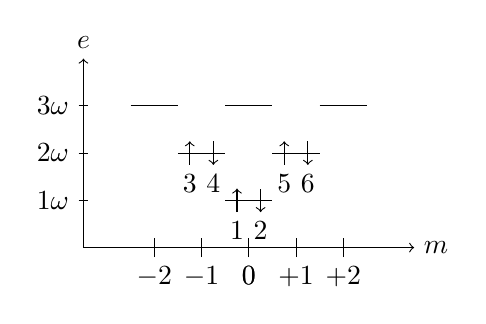
\begin{tikzpicture}[scale=0.6]
  \draw[->] (-3.5,-1) -- (3.5,-1) node[anchor=west] {$m$};
  \draw[->] (-3.5,-1) -- (-3.5,3) node[anchor=south] {$e$};

  \draw (-3.6,0) node[anchor=east] {$1\omega$} -- (-3.4,0);
  \draw (-3.6,1) node[anchor=east] {$2\omega$} -- (-3.4,1);
  \draw (-3.6,2) node[anchor=east] {$3\omega$} -- (-3.4,2);

  \draw (-2,-1.2) node[anchor=north] {$-2$} -- (-2,-.8);
  \draw (-1,-1.2) node[anchor=north] {$-1$} -- (-1,-.8);
  \draw (0,-1.2) node[anchor=north] {$0$} -- (0,-.8);
  \draw (0,-1.2) node[anchor=north] {$0$} -- (0,-.8);
  \draw (1,-1.2) node[anchor=north] {$+1$} -- (1,-.8);
  \draw (2,-1.2) node[anchor=north] {$+2$} -- (2,-.8);

  \begin{scope}
    \draw (-.5,0) -- (.5,0);
    \draw[->] (-.25,-.25) node[anchor=north]{$1$} -- (-.25,.25);
    \draw[<-] (.25,-.25) node[anchor=north]{$2$} -- (.25,.25);
  \end{scope}

  \begin{scope}[xshift=-1cm,yshift=1cm]
    \draw (-.5,0) -- (.5,0);
    \draw[->] (-.25,-.25) node[anchor=north]{$3$} -- (-.25,.25);
    \draw[<-] (.25,-.25) node[anchor=north]{$4$} -- (.25,.25);
  \end{scope}


  \begin{scope}[xshift=1cm,yshift=1cm]
    \draw (-.5,0) -- (.5,0);
    \draw[->] (-.25,-.25) node[anchor=north]{$5$} -- (-.25,.25);
    \draw[<-] (.25,-.25) node[anchor=north]{$6$} -- (.25,.25);
  \end{scope}


  \begin{scope}[xshift=-2cm,yshift=2cm]
    \draw (-.5,0) -- (.5,0);
    %\draw[->] (-.25,-.25) node[anchor=north]{$7$} -- (-.25,.25);
    %\draw[<-] (.25,-.25) node[anchor=north]{$8$} -- (.25,.25);
  \end{scope}


  \begin{scope}[xshift=0cm,yshift=2cm]
    \draw (-.5,0) -- (.5,0);
    %\draw[->] (-.25,-.25) node[anchor=north]{$9$} -- (-.25,.25);
    %\draw[<-] (.25,-.25) node[anchor=north]{$10$} -- (.25,.25);
  \end{scope}


  \begin{scope}[xshift=2cm,yshift=2cm]
    \draw (-.5,0) -- (.5,0);
    %\draw[->] (-.25,-.25) node[anchor=north]{$11$} -- (-.25,.25);
    %\draw[<-] (.25,-.25) node[anchor=north]{$12$} -- (.25,.25);
  \end{scope}
\end{tikzpicture}
\caption{Ground state of the non-interacting problem, the reference Slater determinant $|\Phi\rangle$ for the six-electron system. The electrons occupy the $\u{1}$, $\d{1}$, $\u{2}$, $\d{2}$, $\u{3}$, and $\d{3}$ spin-orbitals.}
\label{fig:4}
\end{SCfigure}
For six electrons, the reference Slater determinant is $|\Phi\rangle = |\u{1}\d{1}\u{2}\d{2}\u{3}\d{3}\rangle$, i.e. the one with spatial orbitals $(n=0,m=0)$, $(n=0,m=-1)$, and $(n=0,m=1)$ occupied. We note that the energy of this Slater determinant under the non-interacting Hamiltonian is $E_0^{(6)}=10$, and the fermi level is now at $E_f^{(6)}=2$ (the energy of the spin-orbitals $\u{2}$, $\d{2}$, $\u{3}$, and $\d{3}$). The reference state is shown in \fig{4} in so called Fock-Darwin representation.

In the same was as for the two-electron case, we can calculate the reference energy using our algorithm (the script should be general enough to handle both cases). The result, $E_\text{ref}^{(6)}=22.2198$, is not great. We note that the relative error in this approximation of the ground state energy (taking $E_0$ to be the \emph{true} ground state energy now) is $10.2\%$. In comparison, the relative error in the approximation in the two-electron case was $8.4\%$. 

For the six-electron case, we still demand $S_z=M=0$ which means we are still restricted to the exact same allowed one-particle-one-hole excitations, namely $\u{1}\rightarrow \u{5}$ and $\d{1}\rightarrow\d{5}$. Because of this, extending the CIS part of the script to the six-electron case requires next to no extra work. Setting up the matrix, and diagonalizing it yields
\begin{align}
H_\text{CIS}^{(6)} = \bmat{ccc}{22.2198    & 0.7833    & 0.7833 \\
0.7833  & 23.4757   & 0.1762 \\
0.7833  &  0.1762  & 23.4757},
\end{align}
and $E_\text{CIS}^{(6)}=21.6168$, which is an improvement over the reference, but as in the two-electron case, still not great. However, the same restrictions as before apply here also, and we have done (just about) no extra work to make it happen, so I guess we should be happy here also. Before we turn to the next exercise we note that the relative errors of the CIS energy is $5.2\%$ and $7.2\%$ for the two-, and six-electron cases respectively.

\subsection*{Exercise 3}
Having treated the parabolic quantum dot with con guration-interaction, we now turn to a restricted Hartree–Fock (RHF) treatment.
\begin{exframe}
\begin{itemize}
  \item[3a)] Define the RHF wavefunction $|\Phi_\text{RHF}\rangle$ for an even number of particles. Use the notation $\tilde{\psi}_I({\bf r})$, for $I=1,2,3,\dots,N/2$, for the unknown spatial orbitals to be found. 

  Compute, in terms of the unknown orbitals, 
  \begin{align}
  E_\text{RHF} = \langle \Phi_\text{RHF} | \hat{H} | \Phi_\text{RHF}\rangle,
  \end{align}
  and compare with general HF.
\end{itemize}
\end{exframe}
The restricted Hartree-Fock wavefunction is a single Slater ansatz for the \emph{true} wavefunction, where each spatial orbital is occupied by exactly two electrons. The wavefunction thus takes the form
\begin{align}
|\Phi_\text{RHF}\rangle &= |\tilde{\psi}_{1,-1}\tilde{\psi}_{1,+1} \tilde{\psi}_{2,-1}\tilde{\psi}_{2,+1}\dots \tilde{\psi}_{N/2,-1}\tilde{\psi}_{N/2,+1} \rangle,
\end{align}
where the subscripts, $(p, \alpha)$ denote the spatial orbital index $p$, and the spin projection, $\alpha$, of the spin-orbitals. We note that all spatial orbitals are "paired," with two occupying electrons, yielding a system with pair-wise equal spatial orbitals.

Applying the Hamiltoninan to this state, we find
\begin{align}
\langle \Phi_\text{RHF} | \hat{H} | \Phi_\text{RHF} \rangle &= \sum_{\alpha=\pm1} \sum_{i=1}^{N/2} \langle \tilde{\psi}_{i,\alpha} | \hat{h} | \tilde{\psi}_{i,\alpha}\rangle + \sum_{\alpha=\pm1}\sum_{i=1}^{N/2}\sum_{\beta=\pm1}\sum_{j=1}^{N/2} \langle \tilde{\psi}_{i,\alpha} \tilde{\psi}_{j,\beta} | \hat{w} | \tilde{\psi}_{i,\alpha} \tilde{\psi}_{j,\beta} - \tilde{\psi}_{j,\beta}\tilde{\psi}_{i,\alpha}\rangle \nn\\
%
&= 2\sum_{i=1}^{N/2} (\tilde{\psi}_i | \hat{h} | \tilde{\psi}_i) + 2\sum_{i=1}^{N/2}\sum_{j=1}^{N/2} (\tilde{\psi}_i \tilde{\psi}_j | \hat{w} | \tilde{\psi}_i \tilde{\psi}_j) -  \sum_{i=1}^{N/2}\sum_{j=1}^{N/2}(\tilde{\psi}_i \tilde{\psi}_j | \hat{w} | \tilde{\psi}_j\tilde{\psi}_i),\label{eq:7}
\end{align}
where we denote by $(\cdot|\cdot)$ the spatial matrix element after the spin-part of the the wavefunction has been factorized out.

For canonical Hartree-Fock, we may find $\langle \Phi | \hat{H} | \Phi\rangle$ by left-multiplying the Hatree-Fock equation, $\hat{f}(\phi_1,\phi_2,\dots,\phi_N)|\phi_i\rangle = \varepsilon_i |\phi_i\rangle$, by $\sum_{i=1}^N\langle \phi_i|$. Doing this yields 
\begin{align}
E_\text{HF} &= \sum_{i=1}^N\langle \phi_i|\hat{h}+\hat{\nu}^\text{direct} - \hat{\nu}^\text{exchange}|\phi_i\rangle \nn\\
&= \sum_{i=1}^N\langle \phi_i|\hat{h}|\phi_i\rangle + \sum_{i=1}^N\sum_{j=1}^N\langle \phi_i\phi_j|\hat{w}|\phi_i\phi_j\rangle - \sum_{i=1}^N\sum_{j=1}^N\langle \phi_i\phi_j|\hat{w}|\phi_j\phi_i\rangle. \label{eq:8}
\end{align}
Eqs. (\ref{eq:7}) and (\ref{eq:8}) look similar, but have a few crucial differences, first and foremost of which is the fact that in the former we have factored out the spin parts of the wavefunction and we have only half as many orbitals (canonical Hartree-Fock spin-orbitals are not required to have pair-wise equal spatial parts).

\begin{exframe}
\begin{itemize}
  \item[3b)] In the remainder, we limit ourselves to $N=2$ and $N=6$. We expand the RHF spatial orbitals in the harmonic oscillator functions, $\psi_p({\bf r})$ for $p=1,2,\dots,6$. Define a $6\times6$ matrix $U$ and write
  \begin{align}
  \tilde{\psi}_p({\bf r})U_{pq}. \label{eq:9}
  \end{align}
  Explain why the matrix $U$ must be unitary. What part of $U$ corresponds to the occupied RHF orbitals? What part corresponds to the virtual RHF orbitals?
\end{itemize}
\end{exframe}
The matrix $U$ is not unitary in general, but it will be if the basis used is orthonormal. In general, $U^\dagger S U = \mathbb{1}$, with $S$ being the overlap matrix and $\mathbb{1}$ being the identity matrix. Since our basis is orthonormal, we can show that $U$ must be unitary. Let us take 
\begin{align}
|\tilde{\psi}_q\rangle = \sum_{p=1}^6 |{\psi}_q\rangle U_{pq},
\end{align}
and left-multiply by the Hermitian conjugate, giving
\begin{align}
\langle \tilde{\psi}_{q'}|\tilde{\psi}_q\rangle &= \sum_{p=1}^6 \langle\tilde{\psi}_{q}|{\psi}_p\rangle U_{pq} \nn\\
\delta_{q'q} &=\sum_{p'=1}^6\sum_{p=1}^6 U^*_{q'p'}\underbrace{\langle\psi_{p'}|{\psi}_p\rangle}_{\delta_{p'p}} U_{pq} \nn\\
 \mathbb{1} &= \sum_{p'=1}^6\sum_{p=1}^6 \delta_{p'p} U^*_{q'p'} U_{pq} \nn\\
 &= \sum_{p=1}^6 U^*_{q'p}U_{pq} = U^\dagger U.
\end{align}

The matrix $U$ contains the coefficients of the unknown orbitals, $\tilde \psi_q$, expanded in the basis of the known $\psi_p$. Specifically, column $q$ contains the coefficients for the unkown $\tilde\psi_q$. The first $N$ orbitals are usually called occupied, while the remaining are called virtual. For the two-electron case, we note that the first column of $U$ correspond to the occupied orbitals, while colums from 2 up to and including 6 correspond to the virtual orbitals.

\begin{exframe}
\begin{itemize}
  \item[3c)] Using your result in 3a) and the definition in \eq{9}, show that the RHF energy can be written 
  \begin{align}
  E_\text{RHF} = 2\sum_p\sum_q\sum_i U^*_{qi} (\psi_q|\hat{h}|\psi_p) + 2\sum_p\sum_q\sum_i U^*_{pi} \left(\sum_r\sum_s D_{sr} [qr|ps]\right)U_{pi}. \label{eq:10}
  \end{align}
  The sums over $i$ and $j$ go from $1$ to $N/2$, and we have defined 
  \begin{align}
  [qr|ps] = (\psi_q\psi_r|\hat{w}|\psi_p\psi_s) - \frac{1}{2}(\psi_q\psi_r|\hat{w}|\psi_s\psi_p). 
  \end{align}
  We have also defined the reduced density matrix,
  \begin{align}
  D_{sr} = 2\sum_i U_{si}U^*_{ri}.
  \end{align}
\end{itemize}
\end{exframe}
Taking the energy expression we found in 3a), \eq{7}, and expressing it in terms of the harmonic oscillator basis functions, we find for the first term 
\begin{align}
E_\text{RHF}^{(\text{first term})} &= 2\sum_{i=1}^{N/2} (\tilde{\psi}_i | \hat{h} | \tilde{\psi}_i) \nn\\
&= 2\sum_{p=1}^6 \sum_{i=1}^{N/2} U^*_{pi}({\psi}_p | \hat{h} | {\psi}_p)U_{pi}.
\end{align}
If we consider the second and third terms together, we find
\begin{align}
E_\text{RHF}^{(\text{second+third terms})} &= 2\sum_{i=1}^{N/2}\sum_{j=1}^{N/2} (\tilde{\psi}_i \tilde{\psi}_j | \hat{w} | \tilde{\psi}_i \tilde{\psi}_j) -  \sum_{i=1}^{N/2}\sum_{j=1}^{N/2}(\tilde{\psi}_i \tilde{\psi}_j | \hat{w} | \tilde{\psi}_j\tilde{\psi}_i) \nn\\
%
&= 2\sum_{pqrs}\sum_{i=1}^{N/2}\sum_{j=1}^{N/2}U^*_{qi} U^*_{rj}({\psi}_q {\psi}_r | \hat{w} | {\psi}_p {\psi}_s)U_{pi}U_{sj}   \nn\\
& \ \ \ \ \ \ \ \ \ \ \ -\sum_{pqrs}\sum_{i=1}^{N/2}\sum_{j=1}^{N/2}U^*_{qi} U^*_{rj}({\psi}_q {\psi}_r | \hat{w} | {\psi}_s{\psi}_p)U_{sj}U_{pi} \nn\\
&= 2\sum_{pqrs}\sum_{i=1}^{N/2}\sum_{j=1}^{N/2}\bigg(U^*_{qi} U^*_{rj}({\psi}_q {\psi}_r | \hat{w} | {\psi}_p {\psi}_s)U_{pi}U_{sj}   \nn\\
& \ \ \ \ \ \ \ \ \ \ \ -\frac{1}{2} U^*_{qi} U^*_{rj}({\psi}_q {\psi}_r | \hat{w} | {\psi}_s{\psi}_p)U_{pi}U_{sj}\bigg) \nn\\
&= \sum_{pq}\sum_{i=1}^{N/2} U^*_{qi} \left(2\sum_{rs}\sum_{j=1}^{N/2} U_{sj}U^*_{rj} [qr|ps]\right) U_{pi} \nn\\
&= \sum_{pq}\sum_{i=1}^{N/2} U^*_{qi} \left(\sum_{rs}D_{sr} [qr|ps]\right) U_{pi}, \label{eq:11}
\end{align}
where we have used that a matrix written in terms of it's indices commute as a complex number (i.e. trivially). Combining the first term with these two yields the result shown in \eq{10}.

\eq{11} may alternatively be written in terms of the direct and exchange energies, as
\begin{align}
\sum_{pq}\sum_{i=1}^{N/2} U^*_{qi} \left(\sum_{rs}D_{sr} [qr|ps]\right) U_{pi} &= \sum_{pq}\sum_{i=1}^{N/2} U^*_{qi} \left(\sum_{rs}D_{sr} \psi_q \left[\hat{\nu}^\text{direct}-\frac{1}{2}\hat{\nu}^\text{exchange} \right] \psi_p \right) U_{pi},
\end{align}
with $\hat{\nu}^\text{direct}$ being defined by $\hat{\nu}^\text{direct} |\psi\rangle = \sum_j \langle \ \cdot \ \phi_j | \hat{w}|\psi \phi_j\rangle$ and the exchange potential, $\hat{\nu}^\text{exchange}$, being defined by $\hat{\nu}^\text{exchange} |\psi\rangle = \sum_j \langle \ \cdot \ \phi_j | \hat{w}| \phi_j\psi\rangle$. These two potentials arise from the minimization of the energy under the orthonormality constraints employed in the Hartree-Fock method. The direct potential can be interpreted as an average of the two-body operator $\hat{w}$ over the coordinates of the other particles, weighted by the "particle density," $\rho({\bf r})=\sum_i|\phi({\bf r})|^2$. This results in a "mean-field potential," in that the interactions between the particles are only considered as an interacting with an average density.

The exchange potential, on the other hand, is not local. I.e. in a point ${\bf r}'$, it depends on the values of the wavefunctions of the other particles are every other point. 

The major difference between the restricted and the canonical Hartree-Fock at this point is that the exchange potential is half that of the canonical case. This is because the $\langle\psi_i\psi_j|\hat{w}|\psi_j\psi_i\rangle$ obtains a $\delta_{\alpha_i\alpha_j}$ when the spin is factored out in the RHF approach, which halves the number of terms which contribute.

\begin{exframe}
\begin{itemize}
  \item[3d)] The RHF equations in the given basis can be written 
  \begin{align}
  F(D)U=U\varepsilon, \ \ \ \ \ \ \ \ \ \text{(Roothan-Hall equation)}
  \end{align}
  where $F(D)$ is the Fock matrix,
  \begin{align}
  F_{qp}(D) = (\psi_q|\hat{h}|\psi_p) + \sum_r\sum_s D_{sr} [qr|ps],
  \end{align}
  and where $\varepsilon=\text{diag}(\varepsilon_1,\varepsilon_2,\dots,\varepsilon_{L/2})$ is a diagonal matrix of eigenvalues.

  Explain in what way the Roothan-Hall equation differs from an ordinary matrix eigenvalue problem.
\end{itemize}
\end{exframe}
Ordinary eigenvalue problems, $A{\bf x}=\lambda {\bf x}$, can be written in terms of an eigenvector matrix, $V$ (where the columns are the eigenvectors of $A$), and a diagonal matrix of eigenvalues, $\Lambda=\text{diag}(\lambda_1, \lambda_2, \dots, \lambda_N)$,  as $AV=\Lambda V$. This problem can be solved directly for a given numerical $A\in\C^{N\times N}$ (by considering the characteristic polynomial if $N$ is small, or by a QR-algorithm if $N$ is large).

The Roothan-Hall equations on the other hand, have an operator matrix, $F(D)$ which depends on it's eigenvectors through $D=D(U)$. Thus the problem really reads $F(U)U=U \varepsilon$, which is a non-linear problem in $U$. This is called a generalized eigenvalue equation. The way we will solve it is to perform so-called SCF iterations, linearizing the problem and solving for each iteration, hopefully yielding a solution which is closer to the \emph{true} solution.

\begin{exframe}
\begin{itemize}
  \item[3e)] Show that the RHF energy can be written 
  \begin{align}
  E_\text{RHF} = 2\sum_i\varepsilon_i - \sum_i\sum_p\sum_q U_{qi}^*\left(\sum_s\sum_r D_{sr}[qr|ps] \right)U_{pi}.
  \end{align}
\end{itemize}
\end{exframe}
Left-multiplying the Roothan-Hall equation by $U^\dagger$, we find
\begin{align}
U^\dagger F(D)U &= U^\dagger U\varepsilon = \varepsilon.
\end{align}
Since the right hand side is diagonal, the product on the left hand side must also be diagonal. Let us now consider the diagonal elements of $U^\dagger F(D) U$,
\begin{align}
\varepsilon_{ii} = \varepsilon_i &= \sum_q\sum_p U^*_{iq}F_{qp}(D)U_{pi} \nn\\
&= \sum_q\sum_p U^*_{iq}\left((\psi_q | \hat{h} | \psi_p) + \sum_r \sum_s D_{sr}[qr|ps] \right)U_{pi},
\end{align}
from which we may extract that
\begin{align}
\sum_i\sum_q\sum_p U^*_{qi}(\psi_q|\hat{h}|\psi_p)U_{pi} &= \sum_i \varepsilon_i - U^*_{qi}\sum_i\sum_r\sum_s D_{sr}[qr|ps] U_{pi}.
\end{align}
Inserting this back into the expression for the RHF energy, we find
\begin{align}
E_\text{RHF} &= 2\sum_{p=1}^6 \sum_{i=1}^{N/2} U^*_{pi}({\psi}_p | \hat{h} | {\psi}_p)U_{pi} + \sum_{pq}\sum_{i=1}^{N/2} U^*_{qi} \left(\sum_{rs}D_{sr} [qr|ps]\right) U_{pi} \nn\\
&= 2\left(\sum_i \varepsilon_i - U^*_{qi}\sum_i\sum_r\sum_s D_{sr}[qr|ps] U_{pi} \right)+ \sum_{pq}\sum_{i=1}^{N/2} U^*_{qi} \left(\sum_{rs}D_{sr} [qr|ps]\right) U_{pi} \nn\\
&= 2\sum_i\varepsilon_i - \sum_i\sum_p\sum_q U^*_{qi}\left( \sum_{sr} D_{sr}[qr|ps]\right) U_{pi}.
\end{align}

\begin{exframe}
\begin{itemize}
  \item[3f)] We are now going to solve the Roothan-Hall equation numerically. Use your favorite programming language and environment. Use comments to document your code and make it readable.

  Write first a subroutine/function/module that, given a reduced
  density matrix $D_0$, computes the corresponding Fock matrix
  $F(D_0)$, and then diagonalizes it.

  Thus, your subroutine should solve the standard eigenvalue problem
  $F(D_0)U = U\varepsilon$ and return $U$ and the diagonal elements of
  $\varepsilon$.

  (A useful check on the sanity of your implementation is that $F$ is
  Hermitian.)
\end{itemize}
\end{exframe}
\begin{exframe}
\begin{itemize}
  \item[3g)] Write a program that performs SCF iterations,
  \begin{equation}
    F(U^{(k-1)}) U^{(k)} = U^{(k)}\epsilon^{(k)},
  \end{equation}
  with $U^{(0)}=I$, the identity matrix.

  You will need approximately 15 iterations for convergence. Measure
  the convergence via
  \begin{equation}
    \delta_k = \max_p\{|\varepsilon^{(k)}_p - \varepsilon^{(k-1)}_p|\}.
  \end{equation}
  Plot $\delta_k$ versus $k$, with $\delta_k$ on a log-axis.
  
  At each iteration $k=1,2,\cdots$, compute $E_\text{RHF}$. Discuss the
  convergence properties.

  Compare the converged RHF energy with the results obtained for CIS,
  and with the numerically exact values listed elsewhere in this project.

  Make sure your program handles both $N=2$ and $N=6$, and that you
  discuss both cases.
\end{itemize}
\end{exframe}
A {\sc Matlab} script which performs these calculations can be found the appendix. The convergence for $N=2$ is plotted in \fig{1}, and we note that a linear behaviour in a semi-log plot means the convergence exibits a power law behaviour (until convergence is reached). The analogous plot for the $N=6$ is ommitted, since it looks basically the same as \fig{1}.
\begin{figure}[h]
\centering
\includegraphics[width=10cm]{convergence1.pdf}
\caption{Convergence of the restricted Hartree-Fock energy for $N=2$. \label{fig:1}}
\end{figure}

The restricted Hartree-Fock energies appear to converge to $E_\text{RHF}^{(2)}=3.1627$ and $E_\text{RHF}^{(6)}=21.5932$, which is close to the CIS energies found earlier, $E_\text{CIS}^{(2)}=3.1570$ and $E_\text{CIS}^{(6)}=21.6168$. We note that the configuration interaction singles approach appears to have worked better than the restricted Hartree-Fock approach for the $N=2$ case, but for the $N=6$ case the opposite is true.

\newpage
\subsection*{Appendix}
This code can be found on \url{https://github.com/mortele/FYS-KJM4480/tree/master/Project1}. Downloading and running can be done by 
\begin{lstlisting}
> git clone git@github.com:mortele/FYS-KJM4480.git
> matlab -nodisplay -nosplash -nodesktop -r "run('exercise2.m')"
\end{lstlisting}
\subsubsection*{A1: Code for exercise 2}
\lstinputlisting[language=Matlab]{exercise2.m}

\newpage
\subsubsection*{A2: Code for exercise 3}
This code can be found on \url{https://github.com/mortele/FYS-KJM4480/tree/master/Project1}. Downloading and running can be done by 
\begin{lstlisting}
> git clone git@github.com:mortele/FYS-KJM4480.git
> matlab -nodisplay -nosplash -nodesktop -r "run('exercise3.m')"
\end{lstlisting}
\lstinputlisting[language=Matlab]{exercise3.m}



\end{document}



% \begin{figure}[p!]
% \centering
% \includegraphics[width=12cm]{<fig>.pdf}
% \caption{\label{fig:1}}
% \end{figure}
 
% \lstinputlisting[firstline=1,lastline=2, float=p!, caption={}, label=lst:1]{<code>.m}

